\documentclass[border=4pt,12pt]{standalone}
% House style for redrawn exam diagrams (diagram-v4: 0.4pt lines, filled -latex arrows, fine dashes; stipple and hatching drawn as real dots/lines (no PDF/SVG patterns, so they render in every browser and at any scale); transparent background). Every figure \input's this.
\usepackage{amsmath,amssymb}
\usepackage{txfonts}
\usepackage{pdfrender,xcolor}
% \halo{text}: label on shading. The shading stops just around each letter's outline (a thin knock-out that follows the
% glyphs, like the papers' typesetting), never a box. Owner: "I don't want a box around the text".
\newcommand{\halo}[1]{\leavevmode\rlap{\pdfrender{TextRenderingMode=2,LineWidth=2.2pt,LineJoinStyle=1,StrokeColor=white,FillColor=white}#1}#1}
\usepackage{tikz,pgfplots}
\pgfplotsset{compat=1.18}
\usetikzlibrary{arrows.meta,calc,angles,quotes,patterns,patterns.meta,intersections,positioning,decorations.markings,shapes.geometric}
% Stipple and hatching are drawn as actual dots / lines clipped to the region (path picture), NOT as pattern fills:
% SVG <pattern> fills vanish or blur when browsers scale the image, so the owner could not see the shading.
% Each dot is a 0.72pt square (keeps SVGs small; reads as a dot at print size). Dots sit on one global staggered grid, so neighbouring regions line up.
\makeatletter
\newdimen\ex@x \newdimen\ex@y \newdimen\ex@xa \newdimen\ex@ya \newdimen\ex@xb \newdimen\ex@yb \newcount\ex@row
\def\exam@stipplecolor{black!75}\def\exam@dotr{0.42pt}\def\exam@dotgap{2.5}
\def\ex@rowdots{\ifdim\ex@x<\ex@xb \pgfpathrectangle{\pgfqpoint{\dimexpr\ex@x-0.36pt\relax}{\dimexpr\ex@y-0.36pt\relax}}{\pgfqpoint{0.72pt}{0.72pt}}\advance\ex@x by \exam@dotgap pt\relax\expandafter\ex@rowdots\fi}
\def\exam@stipple{%
  \pgftransformreset% dots are sized in real points even inside scaled pictures
  \pgfpointanchor{path picture bounding box}{south west}\ex@xa=\pgf@x \ex@ya=\pgf@y
  \pgfpointanchor{path picture bounding box}{north east}\ex@xb=\pgf@x \ex@yb=\pgf@y
  \pgfsetfillcolor{\exam@stipplecolor}\pgfmathsetmacro\ex@h{\exam@dotgap/2}%
  \pgfmathtruncatemacro\ex@r{floor(\ex@ya/\ex@h)-1}\ex@row=\ex@r\relax
  \ex@y=\ex@r\dimexpr\ex@h pt\relax
  \loop\ifdim\ex@y<\ex@yb
    \pgfmathtruncatemacro\ex@c{floor(\ex@xa/\exam@dotgap)-1}\ex@x=\ex@c\dimexpr\exam@dotgap pt\relax
    \ifodd\ex@row \advance\ex@x by \ex@h pt\fi
    \ex@rowdots
    \advance\ex@y by \ex@h pt \advance\ex@row by 1
    \ifnum\numexpr\ex@row-(\ex@row/4)*4\relax=0 \pgfusepath{fill}\fi% flush every 4 rows: bounded TeX memory, few clip copies in the SVG
  \repeat\pgfusepath{fill}}
\newdimen\ex@d
\def\exam@hatch#1{% #1 = 1 for /, -1 for \ ; lines 45 degrees, 3pt apart
  \pgftransformreset
  \pgfpointanchor{path picture bounding box}{south west}\ex@xa=\pgf@x \ex@ya=\pgf@y
  \pgfpointanchor{path picture bounding box}{north east}\ex@xb=\pgf@x \ex@yb=\pgf@y
  \ex@d=\dimexpr\ex@yb-\ex@ya\relax \ex@x=\dimexpr\ex@xa-\ex@d\relax
  \loop\ifdim\ex@x<\ex@xb
    \ifnum#1>0 \pgfpathmoveto{\pgfqpoint{\ex@x}{\ex@ya}}\pgfpathlineto{\pgfqpoint{\dimexpr\ex@x+\ex@d\relax}{\ex@yb}}%
    \else \pgfpathmoveto{\pgfqpoint{\ex@x}{\ex@yb}}\pgfpathlineto{\pgfqpoint{\dimexpr\ex@x+\ex@d\relax}{\ex@ya}}\fi
    \advance\ex@x by 4.24pt
  \repeat
  \pgfsetlinewidth{0.4pt}\pgfsetstrokecolor{black}\pgfusepath{stroke}}
\def\examstipple{\exam@stipple}\def\examhatch{\exam@hatch}\def\examsetstipplecolor#1{\def\exam@stipplecolor{#1}}\def\examsetdotgap#1{\def\exam@dotgap{#1}}
\makeatother
% (legacy pattern kept for old files)
% staggered stipple like the NESA papers' dotted shading
\pgfdeclarepatternformonly{exam stipple}{\pgfpointorigin}{\pgfqpoint{2.2pt}{2.2pt}}{\pgfqpoint{2.2pt}{2.2pt}}{%
  \pgfpathcircle{\pgfqpoint{0.55pt}{0.55pt}}{0.42pt}\pgfpathcircle{\pgfqpoint{1.65pt}{1.65pt}}{0.42pt}\pgfusepath{fill}}
\tikzset{
  every picture/.style={line width=0.6pt, >={Latex[length=2mm,width=1.3mm]}},
  curve/.style={line width=0.6pt},
  open arrow/.style={-{Latex[length=2mm,width=1.3mm]}},  % owner: filled -latex heads everywhere, no open chevrons
  aux/.style={dash pattern=on 2pt off 1.5pt, line width=0.6pt},
  shade/.code={\def\exA{#1}\def\exB{none}\ifx\exA\exB\else\pgfkeysalso{fill=black!18}\fi},
  shade/.default=on,
  shade dots/.style={fill=none, path picture={\examstipple}},
  stipple color/.code={\examsetstipplecolor{#1}},
  stipple gap/.code={\examsetdotgap{#1}},
  shade dense dots/.style={fill=none, stipple gap=1.6, path picture={\examstipple}},
  shade hatch/.style={fill=none, path picture={\examhatch{1}}},
  shade hatch reverse/.style={fill=none, path picture={\examhatch{-1}}},
  shade solid/.style={fill=black},
  pt/.style={circle, fill, inner sep=1.1pt},
  open pt/.style={circle, draw, fill=white, inner sep=1.1pt},
}
\pgfplotsset{
  exam axes/.style={axis lines=middle, axis line style={->}, xlabel={$x$}, ylabel={$y$},
    xlabel style={anchor=west}, ylabel style={anchor=south}, tick label style={font=\small},
    every axis plot/.append style={line width=0.6pt, black}, samples=200, clip=false,
    enlargelimits=false, axis on top},
}

\begin{document}
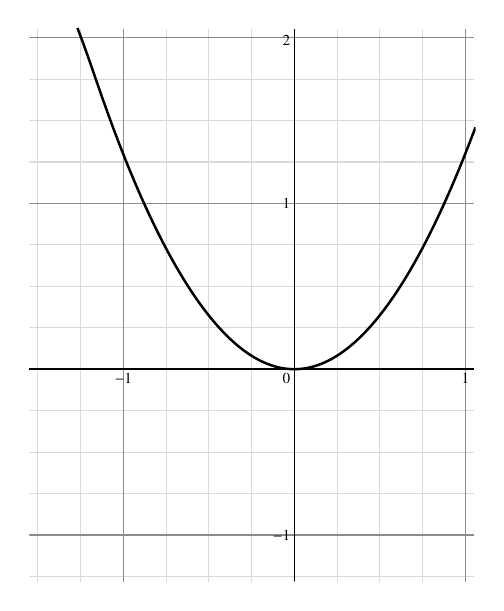
\begin{tikzpicture}[x=2.1717cm,y=2.1057cm]
  % Desmos-style grid: minor lines every 0.25, major every 1 (light grey), axes black, no arrowheads (as the crop)
  \begin{scope}
  \clip (-1.55,-1.28) rectangle (1.05,2.05);
  \draw[black!15,line width=0.4pt] (-1.75,-1.5) grid[step=0.25] (1.25,2.25);
  \draw[black!45,line width=0.5pt] (-2,-2) grid[step=1] (2,3);
  \end{scope}
  \draw (-1.55,0) -- (1.05,0); \draw (0,-1.28) -- (0,2.05);
  \tikzset{tl/.style={font=\fontsize{5.5}{6}\selectfont,inner sep=1.2pt}}
  \node[tl,below] at (-1,0) {$-1$}; \node[tl,below] at (1,0) {$1$}; \node[tl,below left] at (0,0) {$0$};
  \node[tl,left] at (0,1) {$1$}; \node[tl,below left] at (0,2.04) {$2$}; \node[tl,left] at (0,-1) {$-1$};
  % curve traced from the crop (unknown function), fitted as a smoothing spline y(x) (column centres of the stroke)
  \begin{scope}
  \clip (-1.56,-1.29) rectangle (1.06,2.06);
  \draw[line width=0.9pt] plot[smooth] coordinates {(-1.2690,2.0578) (-1.2548,2.0197) (-1.2409,1.9815) (-1.2273,1.9431) (-1.2140,1.9047) (-1.2008,1.8662) (-1.1878,1.8276) (-1.1748,1.7890) (-1.1619,1.7504) (-1.1489,1.7118) (-1.1359,1.6732) (-1.1229,1.6347) (-1.1096,1.5962) (-1.0963,1.5578) (-1.0828,1.5194) (-1.0691,1.4810) (-1.0553,1.4428) (-1.0413,1.4046) (-1.0272,1.3664) (-1.0129,1.3284) (-0.9983,1.2904) (-0.9836,1.2524) (-0.9688,1.2146) (-0.9536,1.1769) (-0.9383,1.1392) (-0.9228,1.1016) (-0.9070,1.0642) (-0.8910,1.0268) (-0.8747,0.9896) (-0.8582,0.9525) (-0.8414,0.9155) (-0.8243,0.8787) (-0.8070,0.8420) (-0.7893,0.8054) (-0.7712,0.7691) (-0.7529,0.7329) (-0.7342,0.6969) (-0.7151,0.6611) (-0.6956,0.6256) (-0.6757,0.5903) (-0.6553,0.5553) (-0.6345,0.5205) (-0.6132,0.4861) (-0.5913,0.4521) (-0.5689,0.4184) (-0.5458,0.3852) (-0.5221,0.3525) (-0.4977,0.3203) (-0.4726,0.2888) (-0.4467,0.2579) (-0.4199,0.2279) (-0.3921,0.1987) (-0.3634,0.1706) (-0.3336,0.1438) (-0.3026,0.1183) (-0.2705,0.0945) (-0.2371,0.0725) (-0.2024,0.0528) (-0.1665,0.0357) (-0.1293,0.0216) (-0.0912,0.0107) (-0.0522,0.0036) (-0.0127,0.0004) (0.0268,0.0012) (0.0661,0.0060) (0.1048,0.0147) (0.1426,0.0270) (0.1792,0.0424) (0.2146,0.0606) (0.2488,0.0812) (0.2817,0.1040) (0.3133,0.1285) (0.3438,0.1546) (0.3731,0.1820) (0.4014,0.2106) (0.4288,0.2401) (0.4552,0.2706) (0.4808,0.3017) (0.5055,0.3336) (0.5296,0.3660) (0.5530,0.3989) (0.5757,0.4324) (0.5979,0.4662) (0.6195,0.5004) (0.6406,0.5350) (0.6612,0.5699) (0.6813,0.6051) (0.7010,0.6405) (0.7203,0.6761) (0.7392,0.7120) (0.7577,0.7481) (0.7759,0.7844) (0.7937,0.8209) (0.8113,0.8575) (0.8285,0.8942) (0.8454,0.9311) (0.8621,0.9682) (0.8785,1.0053) (0.8947,1.0426) (0.9106,1.0800) (0.9263,1.1175) (0.9418,1.1551) (0.9570,1.1928) (0.9721,1.2306) (0.9869,1.2684) (1.0016,1.3064) (1.0161,1.3444) (1.0304,1.3824) (1.0445,1.4206) (1.0585,1.4588)};
  \end{scope}
\end{tikzpicture}
\end{document}
